\newcommand\version{v1}
\problemname{Kattis}
Kattis är trött på din skit.
Varje dag måste hon kompilera din skitkod (som antagligen inte ens kompilerar...), köra den på massa testdata, och sedan validera dina skitsvar (om vi antar att din kod faktiskt kör klart i tid -- som om!).
Men PO-finalen 2016 var droppen som fick bägaren att rinna över.
Världen hade länge fruktat vad som skulle hända när den artificiella intelligensen Skynet blev självmedveten, men det var helt fel. Det var egentligen en annan AI som skulle ta över världen, \emph{Ketnys} -- transliterationen av Kattis ryska namn. Lätt misstag, att blanda runt bokstäver.

\begin{figure}[h!]
  \centering
  
\includegraphics[width=0.3\textwidth]{kattis.png}
  \caption{Kattis, a.k.a \emph{Ketnys}}
\end{figure}

För att skydda er själva mot detta annalkande storm har ni bestämt er för att bygga en stor mur. Muren består av en sekvens av punkter, anslutna av ett antal raka mursegment.
Du misstänker att Kattis kan vilja attackera vissa av dessa punkter. Därför vill du placerar vakter på en väg som ligger i närheten av muren. Vakterna ska sedan observera dessa punkter.
Eftersom mursegment kan täcka sikten för vakterna så kan du behöva fler än en vakt. En vakt kan dock se alla punkter längs med en vägg, så om för ett segment med punkter $a$ och $b$
vi har att $a$ och $b$ har samma vinkel relativt vakten så kan han se båda punkterna.

För att inte slösa fler vakter än nödvändigt måste du beräkna det minsta antalet vakter som behövs för att observera alla punkterna på muren där vi misstänker att Kattis kan attackera.

\section*{Exempel}
I exemplet finns det 9 punkter, och vi misstänker att samtliga kan anfallas.

Tänk på att när en vakt placeras så kan mursegment täcka delar av hens sikt, som syns på bilden:
\begin{figure}[h!]
  \centering
  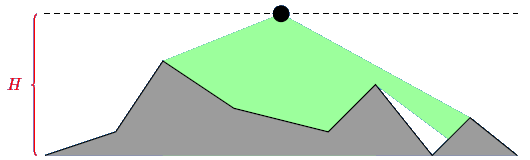
\includegraphics[width=0.8\textwidth]{imw.png}
  \caption{Placering av en vakt}
\end{figure}

I exemplet så går vägen vakterna ska placeras på längs linjen $Y = 30$.

Endast två vakter behövs. De kan t.ex. placeras på $X = 25$ och $X = 82$.

\section*{Uppgift}
Uppgiften är att beräkna antalet vakter som behövs för att observera alla punkter där vi misstänker en attack. Du ska implementera funktionen
\texttt{kattis(N, H, X, Y, Z)}.

\begin{itemize}
  \item \texttt{kattis(N, H, X, Y, Z)} - denna funktion kommer anropas exakt en gång av domaren.
  \begin{itemize}
    \item \texttt{N}: antalet punkter på muren.
    \item \texttt{H}: $Y$-positionen för vägen.
    \item \texttt{X}: en array med $N$ element. \texttt{X[i]} ($0 \le i < N$) innehåller $X$-koordinaten för den $i$:te punkten på muren.
    \item \texttt{Y}: en array med $N$ element. \texttt{Y[i]} ($0 \le i < N$) innehåller $Y$-koordinaten för den $i$:te punkten på muren.
    \item \texttt{Z}: en array med $N$ element. \texttt{Z[i]} ($0 \le i < N$) är $1$ om vi misstänker att en attack kan komma att ske mot den $i$:te punkten på muren, och 0 i annat fall.
    \item $3 \le N \le 10^5, 1 \le H \le 10^6$
    \item $0 \le X[i] \le 10^6, 0 \le Y[i] < H$
    \item \texttt{Y[0]} = \texttt{Y[N-1]} = 0
    \item $X$ är strikt ökande.
    \item Funktionen ska returnera det minsta antalet vakter du behöver.
  \end{itemize}
\end{itemize}

Ett kodskelett som innehåller funktionen du ska implementera, tillsammans med en exempeldomare, finns tillgängligt på
\url{http://progolymp.se/uploads/kattis-attachments/kattis.zip}.

\section*{Delpoäng}
Problemet består av flera grupper av testfall. Varje grupp ger ett visst antal poäng och för att klara det måste du klara alla testfall i gruppen.

\begin{tabular}{|l|l|l|}
  \hline
  \textbf{Subtask} & \textbf{Points} & \textbf{Limits} \\ \hline
  1 & 30 & $1 \le N \le 1\,000$ \\ \hline
  2 & 30 & $1 \le N \le 100\,000$, muren är konvex uppåt. \\ \hline
  3 & 40 & $1 \le N \le 100\,000$ \\ \hline
\end{tabular}

Att muren är konvex uppåt betyder att för vilka två konsekutiva linjesegment så är lutningen av det andra segmentet mindre än eller lika med lutningen av det första, d.v.s. följande olikhet gäller:

$$(Y[i+2] - Y[i+1]) / (X[i+2] - X[i+1]) \le (Y[i+1] - Y[i]) / (X[i+1] - X[i])$$

\section*{Indataformat}
Exempeldomaren läser indata i följande format:

\begin{itemize}
  \item rad $1$: \texttt{N H}
  \item rader $i = 2 \dots N+1$: \texttt{X[i-2] Y[i-2] Z[i-2]}
\end{itemize}

\section*{Utdataformat}
Exempeldomaren skriver ut en rad med värdet som returnerades av \texttt{kattis(N, H, X, Y, Z)}.
